% Chapter Template


\externaldocument{Chapter4}

\chapter{Analysis Methods} % Main chapter title

\label{Chapter5} % Change X to a consecutive number; for referencing this chapter elsewhere, use \ref{ChapterX}

\lhead{Chapter 5 \emph{Preliminary analysis}} % Change X to a consecutive number; this is for the header on each page - perhaps a shortened title



%----------------------------------------------------------------------------------------
%	SECTION 1
%----------------------------------------------------------------------------------------

\section{Data Sorting and Spectrum Extraction}

The first step in the analysis was to extract .spe format spectrum files from the ROOT\cite{root} files which contained the raw data. ROOT is a data analysis package often used with accelerator data. The ROOT data was sorted into a TTree, with data sorted into "leaves", each containing the signals from the MWPC anodes, the scintillators, and the position histogram.

The use of the  scintillator and anode signals was to select the desired reaction. Two of these signals were plotted against each other. The reaction products formed clusters, which could then be selected by a graphical cut. The selection of protons for \textsuperscript{116}Sn(d,p)\textsuperscript{117}Sn is shown in Figure~\ref{rootCut}.

\begin{figure}[h]	
\hspace*{-0.5cm}
\begin{center}	
	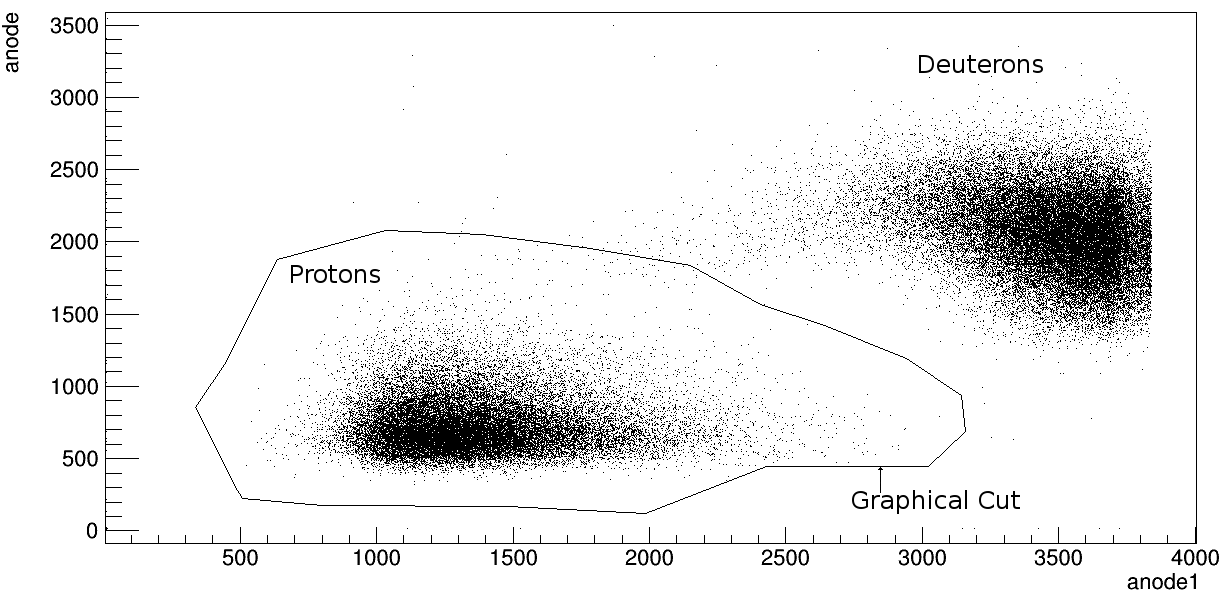
\includegraphics[scale=0.3]{rootcut}
\end{center}
			\caption[Using ROOT cuts for reaction selection]{The two MWPC anode signals plotted against each other for a deuteron beam on a \textsuperscript{116}Sn target. The signals from scattered deuterons and protons are in clusters, so can be separated by a graphical cut. }
		\label{rootCut}
\end{figure}
\FloatBarrier


Once each graphical cut was applied, the position histogram containing all of the counts in the cut was saved to a .spe spectrum format.

\section{Cross-Section Extraction}

The formula for determining the differential cross-section of a reaction from a yield $Y$ is

\begin{equation} \label{eq:yieldxsection}
\frac{\mathrm{d}\sigma}{\mathrm{d}\Omega} = \frac{Y}{\#t\#b\Delta\Omega\varepsilon},
\end{equation}

where $\#t$ is the number of target nuclei per unit area, $\#b$ is the integrated number of beam nuclei, $\Delta\Omega$ is the acceptance solid angle of the spectrograph, and $\varepsilon$ is a dead time correction to the beam current.

To calculate the cross-section for each reaction to each populated state, the corresponding yields were extracted from the spectra, and the other parameters also calculated. $\#b$ was measured by a Brookhaven Instruments Corporation beam current integrator (BIC)\cite{bic}. $\varepsilon$ was calculated by counting the fraction of events in the zero channel of the spectrum.

\subsection{Yield Extraction}

The yields for each state were extracted from the position spectrum by fitting each peak in the spectrum, and finding the area under the fitted curve by integrating it. The ansatz for the fitting was a skewed Gaussian function. The form of a skewed Gaussian function is the sum of a large Gaussian function and a smaller, offset Gaussian function to model the tails seen in the peaks. The fitting was done using the gf3 software from the Radware software package\cite{radware}. An example of a fit is shown in Figure~\ref{gf3Fit}.

\begin{figure}[h]	
\hspace*{-0.5cm}
\begin{center}	
	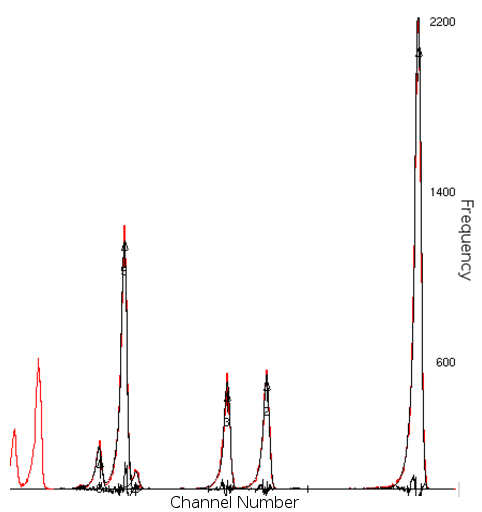
\includegraphics[scale=0.7]{gf3fit}
\end{center}
			\caption[Example fit curve of a spectrum]{An example of a set of peaks which have been fitted with skewed Gaussian fuunctions. This is for \textsuperscript{116}Cd(p,d)\textsuperscript{115}Cd, and the rightmost state is the \textsuperscript{115}Cd ground state. The peaks go from right to left in excitation energy. The red line is the spectrum histogram and the red line is the fitted line. The residuals are also shown. }
		\label{gf3Fit}
\end{figure}
\FloatBarrier

\subsection{Target Thickness}

The $\Delta\Omega$ and $\#t$ terms in Equation~\ref{eq:yieldxsection} were calculated together by using the elastic scattering measurements with the known Rutherford cross-section as discussed in Chapter 4. Because neither term changed between measurements for a specific target, they were substituted back into Equation~\ref{eq:yieldxsection} directly. However, a nominal aperture of \SI{14}{\milli\steradian} was used to approximate the target thickness. This nominal target thickness was then compared to the specification to check for defective foils.

\section{Energy Calibration}

The position of a peak along the spectrograph was proportional to the average momentum of the reaction products which composed the peak. The kinetic energy of these reaction products was proportional to the square of the momentum. There was a negative linear relationship between the kinetic energy of the reaction products and the excitation energy in the residual nucleus.

Overall, there was a negative quadratic relationship between the position of a peak along the focal plane and the excitation energy. Because of this, the ground state of the residual nucleus was always the rightmost peak. From here, the first few strong excited states were identified. The positions of these states were plotted against the energy, and a quadratic fit was made to the data.

Known, strong excited states of higher energy were identified by extrapolating this quadratic fit. This was done recursively, because the errors became very large quickly for the extrapolation, so identification became unreliable away from the known states. The energies of weaker states, unknown states, and previously unresolved doublets were calculated by interpoating the final fit. A calibration for the lowest lying states in \textsuperscript{117}Cd is shown in Figure~\ref{energyCalibration}.


\begin{figure}[h]	
\hspace*{-0.5cm}
\begin{center}	
	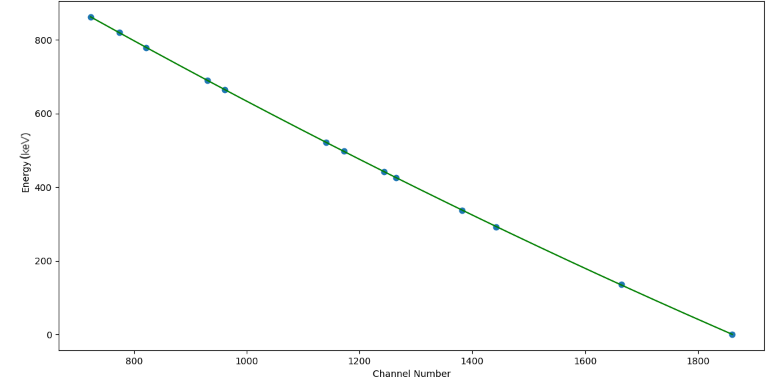
\includegraphics[width=\textwidth]{energycalibration}
\end{center}
			\caption[Energy calibration of the position spectrum]{The energy calibration for the measurement of the lowest MeV of states in \textsuperscript{117}Cd, from \textsuperscript{116}Cd(d,p)\textsuperscript{117}Cd measured at 18 degrees. A full error analysis has not been completed yet, but without errors this method still suffices for the identification of known states. The energies from the fit differ by approximately \SI{1}{\kilo\electronvolt} from previous data for strong states, which sets an approximate uncertainty on any energies calculated by this.}
		\label{energyCalibration}
\end{figure}
\FloatBarrier

The focal plane does not cover all of the energy region of interest, so several measurements were taken with an energy overlap, as discussed in Chapter 4. The overlap allowed the lowest lying states for measurements at higher energies to be identified.

\section{Angular Distributions and $\ell$  Assignment}

To find the occupancies for a given shell, the spectroscopic factors of all states of a given $j$ must be summed. The $\ell$  of each state must therefore be identified. This was done by measuring the angular distribution of the state. The angular distributions are distinct for different $\ell$, with peaks in the differential cross-section at different angles, as discussed in Chapter~\ref{Chapter4}.

The angular distributions for each value of $\ell$ were calculated. This was done by DWBA calculations using the PTOLEMY software\cite{ptolemy}. These distributions were compared to the experimental angular distributions. The experimental distribution was the same fraction smaller for each angle, so the entire calculated distribution was normalised by a constant value $N$, selected to minimize the $\chi^2$. The expression for $N$ for $n$ angle measurements was 

\begin{equation}
N = \frac{ 2 \sum_{i = 1}^{n} \sigma_i \, (\sigma_{i}^{\mathrm{DWBA}}) {}^2 \, s_i^{-2} } {\sum_{j = 1}^{n} \sigma_{j}^{\mathrm{DWBA}} s_j^{-2}}\mathrm{,}
\end{equation}

where $\sigma$ are the measured differential cross-sections, $\sigma^{\mathrm{DWBA}}$ are the cross-sections calculated by DWBA, and $s$ are the uncertainties on the measured cross-sections.

For each state, the normalised angular distributions for each $\ell$ were plotted on the same axes as the measured cross-sections. The $\chi^2$ was also displayed for each fitted distribution with a $\chi^2$ below double that of the fit with the lowest $\chi^2$. The angular momentum was then determined by comparing the value of the fit to the cross-section at the peak of the distribution, the $\chi^2$, and any previous $\ell$ assignment of the state. An example of an angular distribution comparison is shown in Figure~\ref{lAssignment}.

\begin{figure}[h]	
\hspace*{-0.5cm}
\begin{center}	
	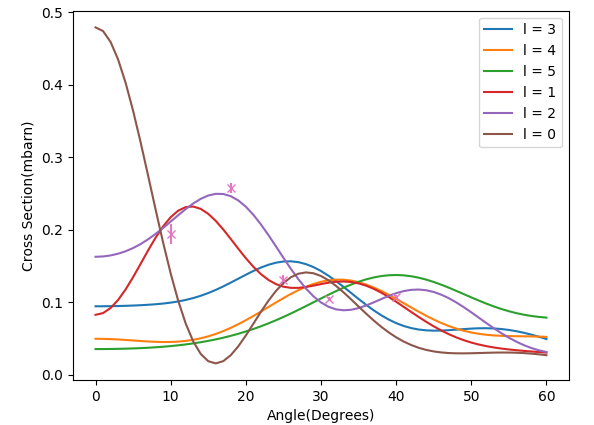
\includegraphics[scale = 0.75]{lassignment}
\end{center}
			\caption[Example of DWBA angular distributions normalised to a measured distribution ]{An example of an angular distribution compared to normalised DWBA distributions. This distribution is for \textsuperscript{116}Cd(d,p)\textsuperscript{117}Sn at a state of 522keV excitation energy. It was assigned as an $\ell = 2$ state.}
		\label{lAssignment}
\end{figure}
\FloatBarrier

\section{Spectroscopic Factors and Sum Rules}

The final section of the analysis will be to extract the spectroscopic factors from the distributions and to calculate the occupancies and vacancies using the Macfarlane and French sum rules. This has not been attempted yet. The cross-section at the peak of each distribution will be divided by the DWBA cross-section at that angle. This will be the spectroscopic factor for each state. Each state will be sorted by its $\ell$, and an occupancy or vacancy will be calculated for each orbital by summing all of the spectroscopic factors for that orbital. This will be normalized to account for missing strength at higher excitation energies. This will be done such that the normalized occupancies and vacancies will sum to $2j + 1$.

\section{Preliminary Assignments}

So far, a full energy calibration has only been done for \textsuperscript{116}Cd(d,p)\textsuperscript{117}Cd, for energies up to \SI{1.2}{\mega\electronvolt}. Angular distributions have been extracted for the states in this region. As well as this, the three states of lowest energy in \textsuperscript{116}Cd(p,d)\textsuperscript{117}Cd have also been measured.

The first three states of the (p,d) had angular distributions which closely resemble the theory. The $\ell = 5$ state was not as accurate because of the poor momentum matching for this reaction. These distributions are shown in Figure~\ref{pdDistributions}.


\begin{figure}[h]	
\hspace*{-0.5cm}
\begin{center}	
	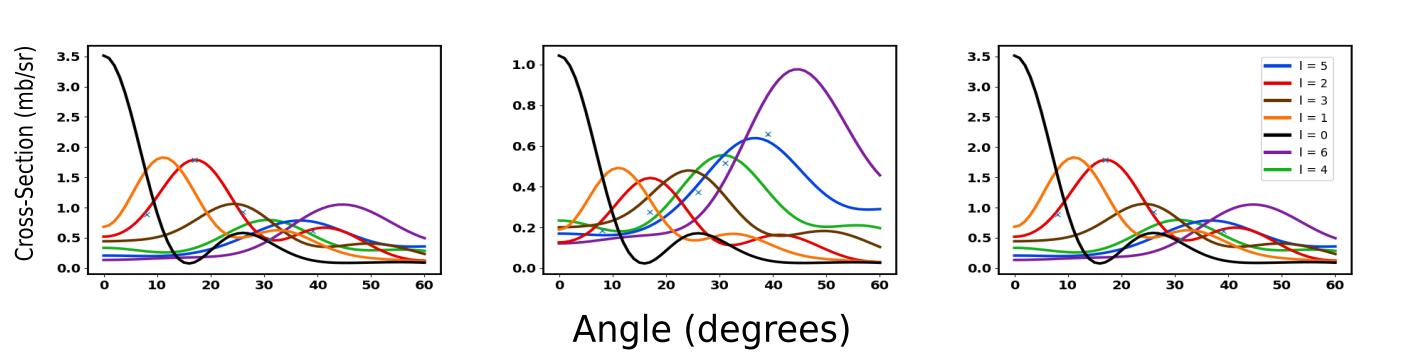
\includegraphics[width  = \textwidth]{pd}
\end{center}
			\caption[\textsuperscript{116}Cd(p,d)\textsuperscript{115}Cd angular distributions for the strongest states ]{Angular distributions for the he first three states in \textsuperscript{115}Cd. These have $\ell = 0,5,2$ respectively.}
		\label{pdDistributions}
\end{figure}
\FloatBarrier

For the (d,p), the distributions did not fit as well, particularly for $\ell = 0$ states. They were still identifiable, but the poor fit means that the spectroscopic factors for these graphs will be unreliable. The $\ell = 2$
fit the distributons well, as in Figure~\ref{lAssignment}. All of the angular distributions for (d,p), with all of the  possible theoretical distributions for each $\ell$ , are shown in Figure~\ref{dpDistributions}.

\begin{figure}[h]	
\vspace*{-2cm}
    \makebox[\linewidth]{
        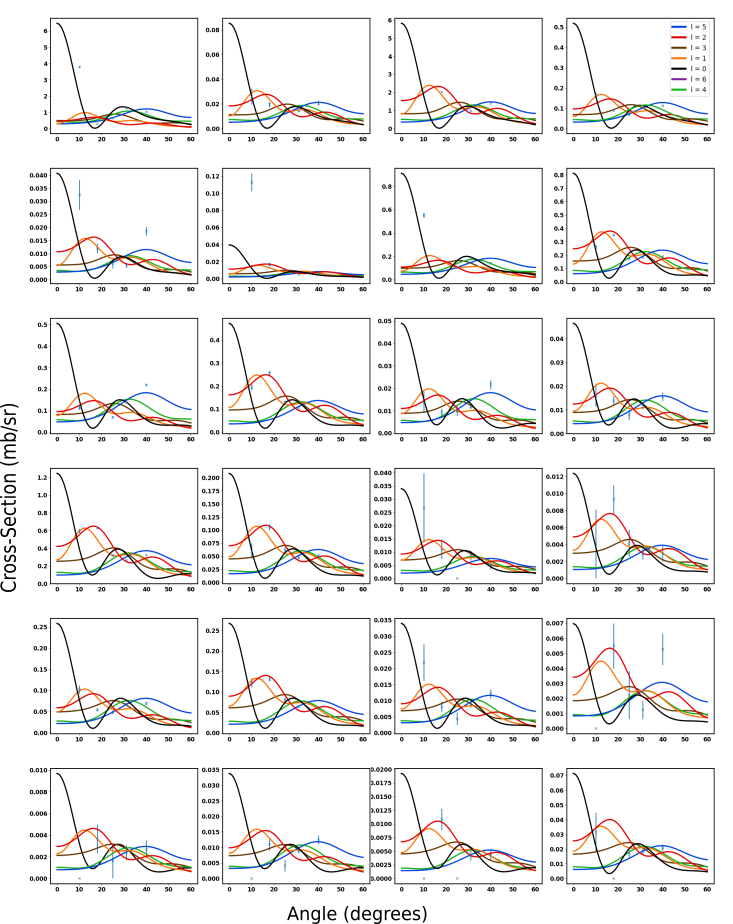
\includegraphics[width=1.3\linewidth]{dp}	
		}
			\caption[The angular distributions for (d,p) reactions to states in \textsuperscript{117}Cd]{The angular distributions for (d,p) to states in \textsuperscript{117}Cd. These are up to 1.2 MeV in excitation energy. For $\ell = 0$ states, The DWBA cross-sections do not match the experimental cross-sections very well.}
		\label{dpDistributions}
\end{figure}
\FloatBarrier


The cross-sections for the (d,p) on \textsuperscript{116}Sn did not match with previous measurements\cite{stuart}. Early results from another recent experiment to check these measurements were consistent with the earlier measurements rather than those discussed in this report. The entirety of the (d,p) data may have been incorrect. This will be verified if the normalisation for occupancies and vacancies for \textsuperscript{116}Cd match the tin.